\chapter{\textit{Universal Filter Multi Carrier} - UFMC} \label{capitulo4}

\chapter{\textit{Filter Bank Multicarrier} - FBMC} \label{capitulo3}

%Este capítulo descreve as principais formas de onda candidatas a 5G. O OFDM já é bastante conhecido, então será apresentado de forma breve, dando-se destaque as suas variações, citadas no capítulo anterior. O FBMC e o UFMC são trazidos de forma detalhada, mostrando-se, inclusive, o comportamento dessas formas de onda sob efeitos do canal de comunicação RF. 

%\section{Orthogonal Fequency Division Multiplexing (OFDM)}

%\begin{figure}[h!]
%\centering
%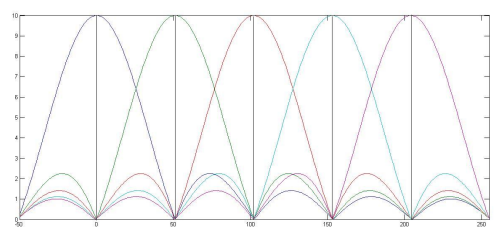
\includegraphics[width=3.5in]{fig_OFDM_freq.png}
%\caption{Subportadoras OFDM}
%\label{fig_OFDM_freq.png}
%\end{figure}
%\end{figure}

%\section{Filter Bank Multi Carrier (FBMC)}
A descrição da forma de onda FBMC pode ser vista como uma generalização do OFDM, com menos restrições em relação ao formato de pulso utilizado para filtrar subportadoras. No contexto da 5G, entretanto, trata-se de algo mais robusto. O projeto PHYDAS (\textit{\textbf{PHY}sical layer for \textbf{DY}namic \textbf{A}cces\text{S} and cognitive radio}) \cite{phydas} se preocupou em criar um desenho bastante específico desta tecnologia, procurando construí-la de tal forma que diversas desvantagens do OFDM fossem superadas, abrindo portas para tornar as aplicações idealizadas para a 5G possíveis. É esta versão que será trazida aqui. 


\section{O Formato de Pulso}\label{pulso} 

Como o filtro FBMC é o que o diferencia do OFDM, inicia-se a apresentação da forma de onda através do formato de pulso utilizado. Sabe-se que a IFFT/FFT possui um efeito de filtragem dos sinais a que é aplicada \cite{Boroujeny}. No domínio do tempo (discreto), pode-se representar este efeito da maneira a seguir \cite{Bellanger}:
\begin{equation}
y_{n} = \frac{1}{M}[x(n-M)+...+x(n-1)] = \frac{1}{M}\sum_{i=1}^{M}x(n-1),
\end{equation}
um filtro passa-baixa do tipo FIR (\textit{finite impulse response} - reposta ao impulso finita). No domínio da frequência \cite{Bellanger}:
\begin{equation}\label{eq_freq}
I(f) = \frac{sin\pi fM}{Msin\pi f}
\end{equation}

A equação \ref{eq_freq} é a fórmula matemática que leva ao espectro visto na figura \ref{fig_OFDM_freq}. A existências de lóbulos laterais de relativamente alta potência esbarra em algumas características que a forma de onda que transmitirá sinais 5G precisará ter. Recapitulando, isto é prejudical a sinais assíncronos, visto que representam um alto potencial para gerar interferências e assincronismo será fundamental no contexto da IoT \cite{Wunder}.  
\par Pensando nisso, procurou-se criar um tipo de filtro mais adequado. Baseou-se a escolha do pulso no critério de Nyquist, que no domínio da frequência significa simetria em relação a frequência de corte \cite{Bellanger}. 
\par Focando agora no processo de transmissão e recepção, para que este ocorra livre de erros, o filtro que transmite deve estar casado com aquele que recebe o sinal. Assim, utiliza-se "meio filtro" de Nyquist na saída e outro "meio filtro" na entrada. 
\par Com esses critérios em mente, desenhou-se alguns possíveis formatos para o pulso FBMC, chegando-se aos coeficientes abaixo: 

\begin{center} \label{coef_FBMC}
\begin{tabular}{ c c c c c c  }
 K & $H_{0}$ &  $H_{1}$ & $H_{2}$ & $H_{3}$ & $\sigma^{2}$ (dB) \\ 
 2 & 1 & $\frac{\sqrt{2}}{2}$ & - & - & -35\\  
 3 & 1 & 0.911438 & 0.411438 & - & -44\\
 4 & 1 & 0.971960 & $\frac{\sqrt{2}}{2}$ & 0.235147 & -65
\end{tabular}
\end{center}

Na tabela \ref{coef_FBMC}m, K representa o fator de superposição, ou seja, quantas amostras se sobrepõem em cada versão do filtro. Quanto maior for K, melhor localizado na frequência será o pulso. Para K = 4, tem-se a resposta da figura \ref{fig_FBMC}, no domínio da frequência:

\begin{figure}[h!]
\centering
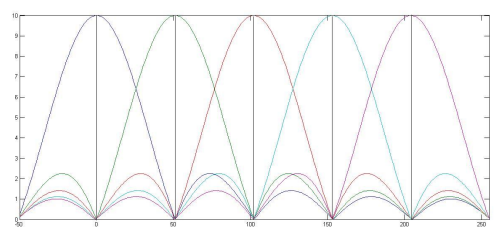
\includegraphics[width=3.5in]{fig_OFDM_freq.png}
\caption{Subportadoras FBMC}
\label{fig_FBMC}
\end{figure}

\par Nota-se uma expressiva redução da amplitude dos lóbulos laterais \cite{Bellanger}, um excelente benefício no contexto M2M. Em termos matemáticos, a forma de pulso se traduz em\cite{Bellanger}: 

\begin{equation}\label{eq_freq}
H(f) = \sum_{k=-(K-1)}^{K-1}H_{k}\frac{\sin(\pi(f-\frac{k}{MK}))}{MKsin(\pi(f-\frac{k}{MK}))}
\end{equation}

\par O próximo passo na construção da forma de onda FBMC é criar múltiplas subportadoras como a da \ref{fig_FBMC}, centralizadas em diferentes frequências. Isto é feito como mostra o diagrama de blocos da figura \ref{Trans_FBMC}. 

\begin{figure}[h!]
\centering
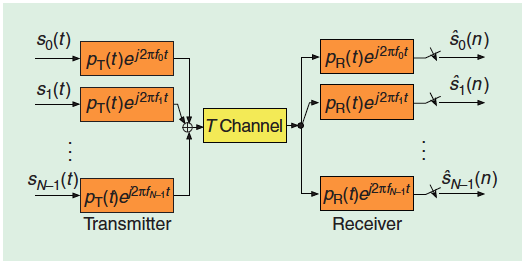
\includegraphics[width=3.5in]{Trans_FBMC.png}
\caption{Diagrama do Modem FBMC \cite{Boroujeny}}
\label{Trans_FBMC}
\end{figure}

\par Na seção do OFDM viu-se o quanto os algortimos de IFFT/FFT foram fundamentais no desenvolvimento da forma de onda tratada ali. Observando-se a Figura \ref{Trans_FBMC}, observa-se uma oportunidade de utilização da ferramenta, já que cada ramo é multiplicado por $\exp^{^{+}_{-} j2\pi}{f_{k}}$, $f_{k} = \frac{ft}{T}$ - coeficientes da transformada de Fourier. 

\par A próxima seção mostra que de fato se pode utilizar a transformada de Fourier para gerar os símbolos FBMC, o que torna a implementação muito mais simples. Para tanto é utilizada um recurso chamado "filtro polifásico". No caso da Figura \ref{Trans_FBMC}, seria necessária a utilização de osciladores de frequência, o que pode dificultar o processo de recepção correta, visto que instrumentos deste tipo são bastante suscetíveis a erros. 

\section{Filtros Polifásicos}

\par Quando se estuda o OFDM, uma das primeiras vantagens que costuma ser ver citada por autores é a facilidade de implementação através dos algoritmos de IFFT/FFT. Viu-se no final da seção anterior que depender de osciladores na frequência é um cenário muito distante do ideal. Filtros polifásicos são a ferramenta que possibilita se distanciar desse contexto analógico, aproximado-se da realidade digital do OFDM. Como construir um banco de filtros através deste recurso é o tema desta seção. 

\par Para entender como funcionam os filtros polifásicos, é necessário entender alguns conceitos de processamento digital de sinais (DSP). O primeiro deles é a decimação ou sub-amostragem. Esta operação consiste em dividir a quantidade de amostras de uma sequência de símbolos por um fator M inteiro e positivo \cite{Krishna}. Matematicamente:

\begin{equation}\label{downsampling}
x_{d}[n] = x[Mn] 
\end{equation}

Visualizar esta operação na frequência é menos intuitivo que no domínio do tempo. Ao se aplicar a transformada de Fourier a uma sequência $x_{c}(t)$ amostrada a $f_{s} = \frac{1}{T}$, obtem-se \cite{Krishna}:

\begin{equation}\label{freq}
X(e^{j\omega}) = \frac{1}{T}\sum_{k = -\infty}^{\infty}X_{c}\bigg[j\bigg(\frac{\omega}{T}-\frac{2\pi k},{T}\bigg)\bigg]
\end{equation}
que é simplesmente a representação espectral de x[n]:

\begin{figure}[h!]
\centering
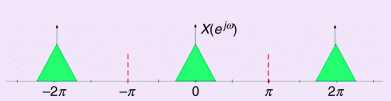
\includegraphics[width=3.5in]{espectro_gen.png}
\caption{Espectro de um Sinal Genérico $x[n]$ \cite{Krishna}}
\label{espec}
\end{figure}

Ao se repetir a operação para uma sequência subamostrada tal qual a que aparece na equação \ref{downsampling}, o resultado será \cite{Krishna}:

\begin{equation}\label{downfreq}
X(e^{j\omega}) = \frac{1}{MT}\sum_{r = -\infty}^{\infty}X_{c}\bigg[j\bigg(\frac{\omega}{MT}-\frac{2\pi r}{MT}\bigg)\bigg]
\end{equation}

\par Aparentemnte, não houve grande alteração em relação ao que foi visto na equação \ref{freq}. Entretanto, substituir-se $r$ em \ref{downfreq} por $m + kM$, em que $ 0 \leq m \leq M-1$ e $-\infty < k < \infty$ leva a \cite{Krishna}:

\begin{equation}\label{downfreq}
X_{d}(e^{j\omega}) = \frac{1}{M}\sum_{m=0}^{M-1}\bigg\{\sum_{k = -\infty}^{\infty}X_{c}\bigg[j\bigg(\frac{\omega-2 \pi m}{MT}-\frac{2\pi k}{MT}\bigg)\bigg]\bigg\},
\end{equation}

que pode ser reescrita, simplesmente como \cite{Krishna}:

\begin{equation}\label{polyfreq}
X(e^{j\omega}) = \frac{1}{M}\sum_{m = 0}^{M-1}X^{\big(e^{j\frac{\omega-2\pi m}{M}}\big)}
\end{equation}

\par Graficamente, a equação \ref{polyfreq} é representada pela figura \ref{downspec} par M = 2. 

\begin{figure}[h!]
\centering
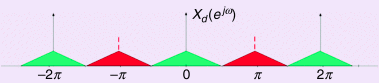
\includegraphics[width=3.5in]{down_espectro_gen.png}
\caption{Espectro de um Sinal Genérico Subamostrado $x_{d}[n]$ \cite{Krishna}}
\label{downespec}
\end{figure}

\par Observa-se que houve uma redução na amplitude do sinal além da sua "multiplicação" espectral. Ainda, nota-se que houve um alargamento da banda em relação à Figura \ref{espectro_gen}. Isso aponta para a necessidade de filtrar o sinal antes de subamostra-lo. Não há muita coerência em aplicar um filtro a amostras que na verdade se deseja descartar. É neste ponto que finalmente se chega ao título desta seção: os filtros polifásicos. Não se deseja que haja \textit{aliasing}, então é fundamental manter-se o processo de filtragem. O filtro polifásico é o recurso que permite que isto seja feito de forma eficiente, como se mostra a seguir: 
\par O processo de filtragem consiste em uma convolução linear \cite{Krishna}: 
\begin{equation}\label{conv}
x[n] = u[n]\ast h[n] = \sum_{k=0}^{N-1} u[k]h[n-k]
\end{equation}
se o produto final é um sinal subamostrado y[n] = x[Mn], a equação \ref{conv} pode ser reescrita como \cite{Krishna}
\begin{equation}\label{conv2}
y[n] = x[Mn] = \sum_{k=0}^{N-1} u[k]h[Mn-k]
\end{equation}
Se, analogamente ao que foi feito em \ref{downfreq}, substituir-se $k$ por $m + rM$, a equação \ref{conv2} se converterá em
\ref{conv} pode ser reescrita como \cite{Krishna}
\begin{equation}\label{conv3}
y[n] = \sum_{m=0}^{M-1}\sum_{r=-\infty}^{\infty} u[rM+m]h[(n-r)M-m]
\end{equation}
\par Pode-se criar uma sequência $u_{m}[r] = u[rM + m]$ e outra $h_{m}[r] = h[rM+m]$, chegando-se a \cite{Krishna}
\begin{equation}\label{conv4}
\begin{split}
y[n] &= \sum_{m=0}^{M-1}\sum_{r=-\infty}^{\infty} u_{m}[r]h[n-r] \\
     &= \sum_{m=0}^{M-1}u_{m}[n]\ast h_{m}[n]
\end{split}
\end{equation}

\par A figura \ref{polifase} ilustra o que acontece com o sinal $u[n]$ quando de uma subamostragem pelo fator M = 4. Esta mostra que somente as amostras importantes participam do processo de convolução (destaque em cores). 

\begin{figure}[h!]
\centering
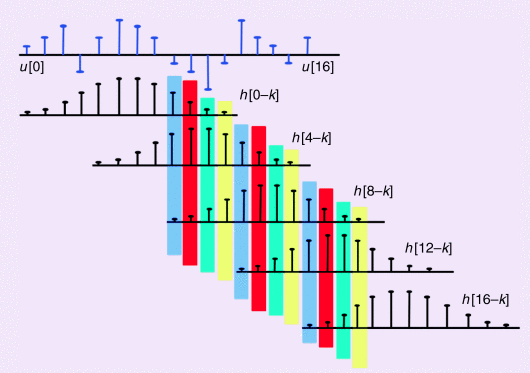
\includegraphics[width=4.5in]{olar.png}
\caption{Convolução por Filtros Polifásicos \cite{Krishna}}
\label{polifase}
\end{figure} 

\par As subsequências formadas por estas amostras são chamadas componentes polifásicas \cite{Krishna}, que se combinadas a transformada de Fourier são capazes de auxiliar no processo de multiplexação de sinais da frequência. Exatemente o que se procura no FBMC. A próxima seção mostra como isso é possível. 

\section{O \textit{Transceptor} FBMC}

\par O FBMC é uma forma de comunicação FDM (\textit{frequency division multiplexing}). Em sistemas deste tipo, vários canais de mesma largura são utilizados para transmissão/recepção de dados \cite{Krishna}, em uma frequência adequada ao tráfego desejado, isto é, em uma posição do espectro que comporte a quantidade de informação que transitará no canal. Comentou-se na seção anterior que esses sistemas, em geral, utilizam de uma arquitetura bastante complexa para detectar o sinal, que depende de osciladores - instrumentos altamente sensíveis a desvios de frequência. Essa tarefa se torna mais simples quando realizada através do processamento digital dos sinais e a estrutura de filtros polifásicos pode servir de grande auxílio neste contexto. 
\par A Figura \ref{polifase2} representa graficamente a equação \ref{conv4} para M = 4. É possível, com o acréscimo de algumas operações algébricas, transformá-la em uma estrutura capaz gerar um sinal de múltiplos canais \ref{Bellanger2}

\begin{figure}[h!]
\centering
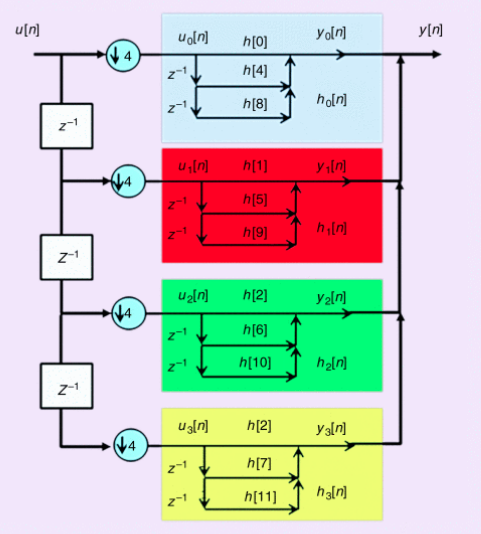
\includegraphics[width=4.5in]{filtro_down.png}
\caption{Convolução por Filtros Polifásicos \cite{Krishna}}
\label{polifase2}
\end{figure} 

Para entender como, é interessante observar a figura \ref{spec_4_chan}

\begin{figure}[h!]
\centering
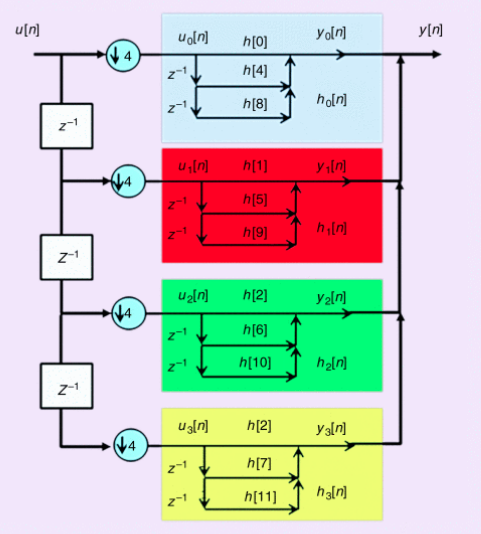
\includegraphics[width=4.5in]{filtro_down.png}
\caption{Convolução por Filtros Polifásicos \cite{Krishna}}
\label{polifase3}
\end{figure} 

Esta figura representa um sinal recebido em um esquema FDM. Ao passa-lo pela estrutura vista na figura \ref{polifase2}, o resultado observado ao final de cada ramo destacado em cores será o que se vê  na Figura \ref{polifase4}. 

\begin{figure}[h!]
\centering
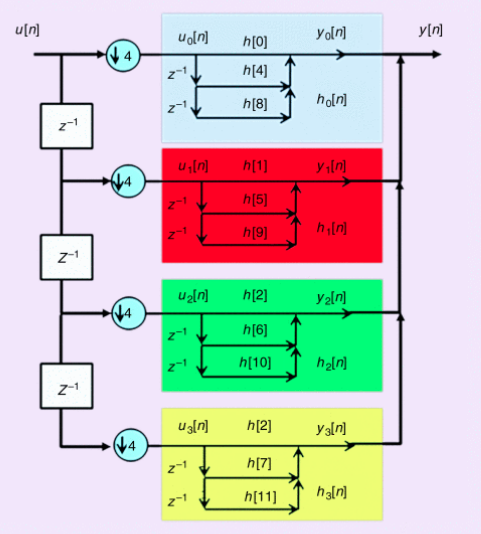
\includegraphics[width=4.5in]{filtro_down.png}
\caption{Convolução por Filtros Polifásicos \cite{Krishna}}
\label{polifase4}
\end{figure} 

A simples soma de todos esses símbolos leva a uma sobreposição de sinais impossibilitando a recuperação de cada banda individualmente. 

\begin{itemize}
\item Canais de frequência com a mesma largura de banda
\item Repepção perfeita na ausência de ruído ou outros efeitos externos 
\end{itemize}


\subsection{Modulação O-QAM} 



\section{Desempenho sob o efeito de não linearidades }